% PREAMBLE
\documentclass[11pt]{amsart}
\usepackage[T1]{fontenc}
\usepackage{lmodern}
\usepackage{microtype}
\usepackage{amsmath,amssymb}
\usepackage{mathtools}
\usepackage{graphicx}
\usepackage{booktabs}
\usepackage{array}
\usepackage{tikz}
\usepackage[colorlinks=true,linkcolor=blue!45!black,citecolor=blue!45!black,urlcolor=blue!45!black]{hyperref}
\usepackage[capitalize]{cleveref}

\newtheorem{theorem}{Theorem}[section]
\newtheorem{proposition}[theorem]{Proposition}
\newtheorem{lemma}[theorem]{Lemma}
\newtheorem{corollary}[theorem]{Corollary}
\newtheorem{conjecture}[theorem]{Conjecture}
\theoremstyle{definition}
\newtheorem{definition}[theorem]{Definition}
\newtheorem{fact}[theorem]{Fact}
\theoremstyle{remark}
\newtheorem{remark}[theorem]{Remark}

\newcommand{\vpy}{\texttt{scripts/\allowbreak verify.py}}
\newcommand{\fpy}{\texttt{scripts/\allowbreak figure.py}}

\DeclareMathOperator{\comp}{comp}
\DeclareMathOperator{\fil}{fill}

\emergencystretch=1em
\raggedbottom

\newcommand{\witnessplate}{%
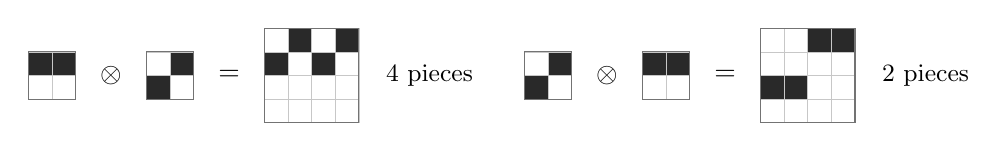
\begin{tikzpicture}[x=1cm,y=1cm]
\fill[black!84] (0.00,0.60) rectangle ++(0.30,0.30);
\fill[black!84] (0.30,0.60) rectangle ++(0.30,0.30);
\fill[white] (0.00,0.30) rectangle ++(0.30,0.30);
\fill[white] (0.30,0.30) rectangle ++(0.30,0.30);
\draw[black!22,line width=0.2pt,step=0.30] (0.00,0.30) grid ++(0.60,0.60);
\draw[black!55,line width=0.4pt] (0.00,0.30) rectangle ++(0.60,0.60);
\node at (1.05,0.60) {$\otimes$};
\fill[white] (1.50,0.60) rectangle ++(0.30,0.30);
\fill[black!84] (1.80,0.60) rectangle ++(0.30,0.30);
\fill[black!84] (1.50,0.30) rectangle ++(0.30,0.30);
\fill[white] (1.80,0.30) rectangle ++(0.30,0.30);
\draw[black!22,line width=0.2pt,step=0.30] (1.50,0.30) grid ++(0.60,0.60);
\draw[black!55,line width=0.4pt] (1.50,0.30) rectangle ++(0.60,0.60);
\node at (2.55,0.60) {$=$};
\fill[white] (3.00,0.90) rectangle ++(0.30,0.30);
\fill[black!84] (3.30,0.90) rectangle ++(0.30,0.30);
\fill[white] (3.60,0.90) rectangle ++(0.30,0.30);
\fill[black!84] (3.90,0.90) rectangle ++(0.30,0.30);
\fill[black!84] (3.00,0.60) rectangle ++(0.30,0.30);
\fill[white] (3.30,0.60) rectangle ++(0.30,0.30);
\fill[black!84] (3.60,0.60) rectangle ++(0.30,0.30);
\fill[white] (3.90,0.60) rectangle ++(0.30,0.30);
\fill[white] (3.00,0.30) rectangle ++(0.30,0.30);
\fill[white] (3.30,0.30) rectangle ++(0.30,0.30);
\fill[white] (3.60,0.30) rectangle ++(0.30,0.30);
\fill[white] (3.90,0.30) rectangle ++(0.30,0.30);
\fill[white] (3.00,0.00) rectangle ++(0.30,0.30);
\fill[white] (3.30,0.00) rectangle ++(0.30,0.30);
\fill[white] (3.60,0.00) rectangle ++(0.30,0.30);
\fill[white] (3.90,0.00) rectangle ++(0.30,0.30);
\draw[black!22,line width=0.2pt,step=0.30] (3.00,0.00) grid ++(1.20,1.20);
\draw[black!55,line width=0.4pt] (3.00,0.00) rectangle ++(1.20,1.20);
\node[anchor=west,font=\small] at (4.42,0.60) {4 pieces};
\fill[white] (6.30,0.60) rectangle ++(0.30,0.30);
\fill[black!84] (6.60,0.60) rectangle ++(0.30,0.30);
\fill[black!84] (6.30,0.30) rectangle ++(0.30,0.30);
\fill[white] (6.60,0.30) rectangle ++(0.30,0.30);
\draw[black!22,line width=0.2pt,step=0.30] (6.30,0.30) grid ++(0.60,0.60);
\draw[black!55,line width=0.4pt] (6.30,0.30) rectangle ++(0.60,0.60);
\node at (7.35,0.60) {$\otimes$};
\fill[black!84] (7.80,0.60) rectangle ++(0.30,0.30);
\fill[black!84] (8.10,0.60) rectangle ++(0.30,0.30);
\fill[white] (7.80,0.30) rectangle ++(0.30,0.30);
\fill[white] (8.10,0.30) rectangle ++(0.30,0.30);
\draw[black!22,line width=0.2pt,step=0.30] (7.80,0.30) grid ++(0.60,0.60);
\draw[black!55,line width=0.4pt] (7.80,0.30) rectangle ++(0.60,0.60);
\node at (8.85,0.60) {$=$};
\fill[white] (9.30,0.90) rectangle ++(0.30,0.30);
\fill[white] (9.60,0.90) rectangle ++(0.30,0.30);
\fill[black!84] (9.90,0.90) rectangle ++(0.30,0.30);
\fill[black!84] (10.20,0.90) rectangle ++(0.30,0.30);
\fill[white] (9.30,0.60) rectangle ++(0.30,0.30);
\fill[white] (9.60,0.60) rectangle ++(0.30,0.30);
\fill[white] (9.90,0.60) rectangle ++(0.30,0.30);
\fill[white] (10.20,0.60) rectangle ++(0.30,0.30);
\fill[black!84] (9.30,0.30) rectangle ++(0.30,0.30);
\fill[black!84] (9.60,0.30) rectangle ++(0.30,0.30);
\fill[white] (9.90,0.30) rectangle ++(0.30,0.30);
\fill[white] (10.20,0.30) rectangle ++(0.30,0.30);
\fill[white] (9.30,0.00) rectangle ++(0.30,0.30);
\fill[white] (9.60,0.00) rectangle ++(0.30,0.30);
\fill[white] (9.90,0.00) rectangle ++(0.30,0.30);
\fill[white] (10.20,0.00) rectangle ++(0.30,0.30);
\draw[black!22,line width=0.2pt,step=0.30] (9.30,0.00) grid ++(1.20,1.20);
\draw[black!55,line width=0.4pt] (9.30,0.00) rectangle ++(1.20,1.20);
\node[anchor=west,font=\small] at (10.72,0.60) {2 pieces};
\end{tikzpicture}}

\newcommand{\ledgerplate}{%
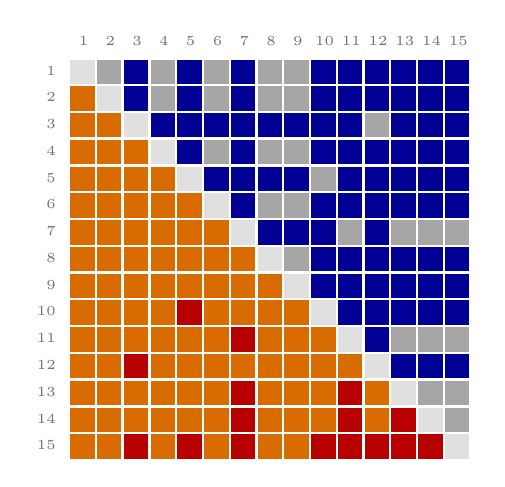
\begin{tikzpicture}[x=1cm,y=1cm]
\node[anchor=east,font=\tiny,text=black!55] at (-0.06,4.93) {1};
\node[anchor=south,font=\tiny,text=black!55] at (0.17,5.12) {1};
\fill[black!12] (0.000,4.760) rectangle ++(0.310,0.310);
\fill[black!35] (0.340,4.760) rectangle ++(0.310,0.310);
\fill[blue!58!black] (0.680,4.760) rectangle ++(0.310,0.310);
\fill[black!35] (1.020,4.760) rectangle ++(0.310,0.310);
\fill[blue!58!black] (1.360,4.760) rectangle ++(0.310,0.310);
\fill[black!35] (1.700,4.760) rectangle ++(0.310,0.310);
\fill[blue!58!black] (2.040,4.760) rectangle ++(0.310,0.310);
\fill[black!35] (2.380,4.760) rectangle ++(0.310,0.310);
\fill[black!35] (2.720,4.760) rectangle ++(0.310,0.310);
\fill[blue!58!black] (3.060,4.760) rectangle ++(0.310,0.310);
\fill[blue!58!black] (3.400,4.760) rectangle ++(0.310,0.310);
\fill[blue!58!black] (3.740,4.760) rectangle ++(0.310,0.310);
\fill[blue!58!black] (4.080,4.760) rectangle ++(0.310,0.310);
\fill[blue!58!black] (4.420,4.760) rectangle ++(0.310,0.310);
\fill[blue!58!black] (4.760,4.760) rectangle ++(0.310,0.310);
\node[anchor=east,font=\tiny,text=black!55] at (-0.06,4.59) {2};
\node[anchor=south,font=\tiny,text=black!55] at (0.51,5.12) {2};
\fill[orange!85!black] (0.000,4.420) rectangle ++(0.310,0.310);
\fill[black!12] (0.340,4.420) rectangle ++(0.310,0.310);
\fill[blue!58!black] (0.680,4.420) rectangle ++(0.310,0.310);
\fill[black!35] (1.020,4.420) rectangle ++(0.310,0.310);
\fill[blue!58!black] (1.360,4.420) rectangle ++(0.310,0.310);
\fill[black!35] (1.700,4.420) rectangle ++(0.310,0.310);
\fill[blue!58!black] (2.040,4.420) rectangle ++(0.310,0.310);
\fill[black!35] (2.380,4.420) rectangle ++(0.310,0.310);
\fill[black!35] (2.720,4.420) rectangle ++(0.310,0.310);
\fill[blue!58!black] (3.060,4.420) rectangle ++(0.310,0.310);
\fill[blue!58!black] (3.400,4.420) rectangle ++(0.310,0.310);
\fill[blue!58!black] (3.740,4.420) rectangle ++(0.310,0.310);
\fill[blue!58!black] (4.080,4.420) rectangle ++(0.310,0.310);
\fill[blue!58!black] (4.420,4.420) rectangle ++(0.310,0.310);
\fill[blue!58!black] (4.760,4.420) rectangle ++(0.310,0.310);
\node[anchor=east,font=\tiny,text=black!55] at (-0.06,4.25) {3};
\node[anchor=south,font=\tiny,text=black!55] at (0.85,5.12) {3};
\fill[orange!85!black] (0.000,4.080) rectangle ++(0.310,0.310);
\fill[orange!85!black] (0.340,4.080) rectangle ++(0.310,0.310);
\fill[black!12] (0.680,4.080) rectangle ++(0.310,0.310);
\fill[blue!58!black] (1.020,4.080) rectangle ++(0.310,0.310);
\fill[blue!58!black] (1.360,4.080) rectangle ++(0.310,0.310);
\fill[blue!58!black] (1.700,4.080) rectangle ++(0.310,0.310);
\fill[blue!58!black] (2.040,4.080) rectangle ++(0.310,0.310);
\fill[blue!58!black] (2.380,4.080) rectangle ++(0.310,0.310);
\fill[blue!58!black] (2.720,4.080) rectangle ++(0.310,0.310);
\fill[blue!58!black] (3.060,4.080) rectangle ++(0.310,0.310);
\fill[blue!58!black] (3.400,4.080) rectangle ++(0.310,0.310);
\fill[black!35] (3.740,4.080) rectangle ++(0.310,0.310);
\fill[blue!58!black] (4.080,4.080) rectangle ++(0.310,0.310);
\fill[blue!58!black] (4.420,4.080) rectangle ++(0.310,0.310);
\fill[blue!58!black] (4.760,4.080) rectangle ++(0.310,0.310);
\node[anchor=east,font=\tiny,text=black!55] at (-0.06,3.91) {4};
\node[anchor=south,font=\tiny,text=black!55] at (1.19,5.12) {4};
\fill[orange!85!black] (0.000,3.740) rectangle ++(0.310,0.310);
\fill[orange!85!black] (0.340,3.740) rectangle ++(0.310,0.310);
\fill[orange!85!black] (0.680,3.740) rectangle ++(0.310,0.310);
\fill[black!12] (1.020,3.740) rectangle ++(0.310,0.310);
\fill[blue!58!black] (1.360,3.740) rectangle ++(0.310,0.310);
\fill[black!35] (1.700,3.740) rectangle ++(0.310,0.310);
\fill[blue!58!black] (2.040,3.740) rectangle ++(0.310,0.310);
\fill[black!35] (2.380,3.740) rectangle ++(0.310,0.310);
\fill[black!35] (2.720,3.740) rectangle ++(0.310,0.310);
\fill[blue!58!black] (3.060,3.740) rectangle ++(0.310,0.310);
\fill[blue!58!black] (3.400,3.740) rectangle ++(0.310,0.310);
\fill[blue!58!black] (3.740,3.740) rectangle ++(0.310,0.310);
\fill[blue!58!black] (4.080,3.740) rectangle ++(0.310,0.310);
\fill[blue!58!black] (4.420,3.740) rectangle ++(0.310,0.310);
\fill[blue!58!black] (4.760,3.740) rectangle ++(0.310,0.310);
\node[anchor=east,font=\tiny,text=black!55] at (-0.06,3.57) {5};
\node[anchor=south,font=\tiny,text=black!55] at (1.53,5.12) {5};
\fill[orange!85!black] (0.000,3.400) rectangle ++(0.310,0.310);
\fill[orange!85!black] (0.340,3.400) rectangle ++(0.310,0.310);
\fill[orange!85!black] (0.680,3.400) rectangle ++(0.310,0.310);
\fill[orange!85!black] (1.020,3.400) rectangle ++(0.310,0.310);
\fill[black!12] (1.360,3.400) rectangle ++(0.310,0.310);
\fill[blue!58!black] (1.700,3.400) rectangle ++(0.310,0.310);
\fill[blue!58!black] (2.040,3.400) rectangle ++(0.310,0.310);
\fill[blue!58!black] (2.380,3.400) rectangle ++(0.310,0.310);
\fill[blue!58!black] (2.720,3.400) rectangle ++(0.310,0.310);
\fill[black!35] (3.060,3.400) rectangle ++(0.310,0.310);
\fill[blue!58!black] (3.400,3.400) rectangle ++(0.310,0.310);
\fill[blue!58!black] (3.740,3.400) rectangle ++(0.310,0.310);
\fill[blue!58!black] (4.080,3.400) rectangle ++(0.310,0.310);
\fill[blue!58!black] (4.420,3.400) rectangle ++(0.310,0.310);
\fill[blue!58!black] (4.760,3.400) rectangle ++(0.310,0.310);
\node[anchor=east,font=\tiny,text=black!55] at (-0.06,3.23) {6};
\node[anchor=south,font=\tiny,text=black!55] at (1.87,5.12) {6};
\fill[orange!85!black] (0.000,3.060) rectangle ++(0.310,0.310);
\fill[orange!85!black] (0.340,3.060) rectangle ++(0.310,0.310);
\fill[orange!85!black] (0.680,3.060) rectangle ++(0.310,0.310);
\fill[orange!85!black] (1.020,3.060) rectangle ++(0.310,0.310);
\fill[orange!85!black] (1.360,3.060) rectangle ++(0.310,0.310);
\fill[black!12] (1.700,3.060) rectangle ++(0.310,0.310);
\fill[blue!58!black] (2.040,3.060) rectangle ++(0.310,0.310);
\fill[black!35] (2.380,3.060) rectangle ++(0.310,0.310);
\fill[black!35] (2.720,3.060) rectangle ++(0.310,0.310);
\fill[blue!58!black] (3.060,3.060) rectangle ++(0.310,0.310);
\fill[blue!58!black] (3.400,3.060) rectangle ++(0.310,0.310);
\fill[blue!58!black] (3.740,3.060) rectangle ++(0.310,0.310);
\fill[blue!58!black] (4.080,3.060) rectangle ++(0.310,0.310);
\fill[blue!58!black] (4.420,3.060) rectangle ++(0.310,0.310);
\fill[blue!58!black] (4.760,3.060) rectangle ++(0.310,0.310);
\node[anchor=east,font=\tiny,text=black!55] at (-0.06,2.89) {7};
\node[anchor=south,font=\tiny,text=black!55] at (2.21,5.12) {7};
\fill[orange!85!black] (0.000,2.720) rectangle ++(0.310,0.310);
\fill[orange!85!black] (0.340,2.720) rectangle ++(0.310,0.310);
\fill[orange!85!black] (0.680,2.720) rectangle ++(0.310,0.310);
\fill[orange!85!black] (1.020,2.720) rectangle ++(0.310,0.310);
\fill[orange!85!black] (1.360,2.720) rectangle ++(0.310,0.310);
\fill[orange!85!black] (1.700,2.720) rectangle ++(0.310,0.310);
\fill[black!12] (2.040,2.720) rectangle ++(0.310,0.310);
\fill[blue!58!black] (2.380,2.720) rectangle ++(0.310,0.310);
\fill[blue!58!black] (2.720,2.720) rectangle ++(0.310,0.310);
\fill[blue!58!black] (3.060,2.720) rectangle ++(0.310,0.310);
\fill[black!35] (3.400,2.720) rectangle ++(0.310,0.310);
\fill[blue!58!black] (3.740,2.720) rectangle ++(0.310,0.310);
\fill[black!35] (4.080,2.720) rectangle ++(0.310,0.310);
\fill[black!35] (4.420,2.720) rectangle ++(0.310,0.310);
\fill[black!35] (4.760,2.720) rectangle ++(0.310,0.310);
\node[anchor=east,font=\tiny,text=black!55] at (-0.06,2.55) {8};
\node[anchor=south,font=\tiny,text=black!55] at (2.55,5.12) {8};
\fill[orange!85!black] (0.000,2.380) rectangle ++(0.310,0.310);
\fill[orange!85!black] (0.340,2.380) rectangle ++(0.310,0.310);
\fill[orange!85!black] (0.680,2.380) rectangle ++(0.310,0.310);
\fill[orange!85!black] (1.020,2.380) rectangle ++(0.310,0.310);
\fill[orange!85!black] (1.360,2.380) rectangle ++(0.310,0.310);
\fill[orange!85!black] (1.700,2.380) rectangle ++(0.310,0.310);
\fill[orange!85!black] (2.040,2.380) rectangle ++(0.310,0.310);
\fill[black!12] (2.380,2.380) rectangle ++(0.310,0.310);
\fill[black!35] (2.720,2.380) rectangle ++(0.310,0.310);
\fill[blue!58!black] (3.060,2.380) rectangle ++(0.310,0.310);
\fill[blue!58!black] (3.400,2.380) rectangle ++(0.310,0.310);
\fill[blue!58!black] (3.740,2.380) rectangle ++(0.310,0.310);
\fill[blue!58!black] (4.080,2.380) rectangle ++(0.310,0.310);
\fill[blue!58!black] (4.420,2.380) rectangle ++(0.310,0.310);
\fill[blue!58!black] (4.760,2.380) rectangle ++(0.310,0.310);
\node[anchor=east,font=\tiny,text=black!55] at (-0.06,2.21) {9};
\node[anchor=south,font=\tiny,text=black!55] at (2.89,5.12) {9};
\fill[orange!85!black] (0.000,2.040) rectangle ++(0.310,0.310);
\fill[orange!85!black] (0.340,2.040) rectangle ++(0.310,0.310);
\fill[orange!85!black] (0.680,2.040) rectangle ++(0.310,0.310);
\fill[orange!85!black] (1.020,2.040) rectangle ++(0.310,0.310);
\fill[orange!85!black] (1.360,2.040) rectangle ++(0.310,0.310);
\fill[orange!85!black] (1.700,2.040) rectangle ++(0.310,0.310);
\fill[orange!85!black] (2.040,2.040) rectangle ++(0.310,0.310);
\fill[orange!85!black] (2.380,2.040) rectangle ++(0.310,0.310);
\fill[black!12] (2.720,2.040) rectangle ++(0.310,0.310);
\fill[blue!58!black] (3.060,2.040) rectangle ++(0.310,0.310);
\fill[blue!58!black] (3.400,2.040) rectangle ++(0.310,0.310);
\fill[blue!58!black] (3.740,2.040) rectangle ++(0.310,0.310);
\fill[blue!58!black] (4.080,2.040) rectangle ++(0.310,0.310);
\fill[blue!58!black] (4.420,2.040) rectangle ++(0.310,0.310);
\fill[blue!58!black] (4.760,2.040) rectangle ++(0.310,0.310);
\node[anchor=east,font=\tiny,text=black!55] at (-0.06,1.87) {10};
\node[anchor=south,font=\tiny,text=black!55] at (3.23,5.12) {10};
\fill[orange!85!black] (0.000,1.700) rectangle ++(0.310,0.310);
\fill[orange!85!black] (0.340,1.700) rectangle ++(0.310,0.310);
\fill[orange!85!black] (0.680,1.700) rectangle ++(0.310,0.310);
\fill[orange!85!black] (1.020,1.700) rectangle ++(0.310,0.310);
\fill[red!72!black] (1.360,1.700) rectangle ++(0.310,0.310);
\fill[orange!85!black] (1.700,1.700) rectangle ++(0.310,0.310);
\fill[orange!85!black] (2.040,1.700) rectangle ++(0.310,0.310);
\fill[orange!85!black] (2.380,1.700) rectangle ++(0.310,0.310);
\fill[orange!85!black] (2.720,1.700) rectangle ++(0.310,0.310);
\fill[black!12] (3.060,1.700) rectangle ++(0.310,0.310);
\fill[blue!58!black] (3.400,1.700) rectangle ++(0.310,0.310);
\fill[blue!58!black] (3.740,1.700) rectangle ++(0.310,0.310);
\fill[blue!58!black] (4.080,1.700) rectangle ++(0.310,0.310);
\fill[blue!58!black] (4.420,1.700) rectangle ++(0.310,0.310);
\fill[blue!58!black] (4.760,1.700) rectangle ++(0.310,0.310);
\node[anchor=east,font=\tiny,text=black!55] at (-0.06,1.53) {11};
\node[anchor=south,font=\tiny,text=black!55] at (3.57,5.12) {11};
\fill[orange!85!black] (0.000,1.360) rectangle ++(0.310,0.310);
\fill[orange!85!black] (0.340,1.360) rectangle ++(0.310,0.310);
\fill[orange!85!black] (0.680,1.360) rectangle ++(0.310,0.310);
\fill[orange!85!black] (1.020,1.360) rectangle ++(0.310,0.310);
\fill[orange!85!black] (1.360,1.360) rectangle ++(0.310,0.310);
\fill[orange!85!black] (1.700,1.360) rectangle ++(0.310,0.310);
\fill[red!72!black] (2.040,1.360) rectangle ++(0.310,0.310);
\fill[orange!85!black] (2.380,1.360) rectangle ++(0.310,0.310);
\fill[orange!85!black] (2.720,1.360) rectangle ++(0.310,0.310);
\fill[orange!85!black] (3.060,1.360) rectangle ++(0.310,0.310);
\fill[black!12] (3.400,1.360) rectangle ++(0.310,0.310);
\fill[blue!58!black] (3.740,1.360) rectangle ++(0.310,0.310);
\fill[black!35] (4.080,1.360) rectangle ++(0.310,0.310);
\fill[black!35] (4.420,1.360) rectangle ++(0.310,0.310);
\fill[black!35] (4.760,1.360) rectangle ++(0.310,0.310);
\node[anchor=east,font=\tiny,text=black!55] at (-0.06,1.19) {12};
\node[anchor=south,font=\tiny,text=black!55] at (3.91,5.12) {12};
\fill[orange!85!black] (0.000,1.020) rectangle ++(0.310,0.310);
\fill[orange!85!black] (0.340,1.020) rectangle ++(0.310,0.310);
\fill[red!72!black] (0.680,1.020) rectangle ++(0.310,0.310);
\fill[orange!85!black] (1.020,1.020) rectangle ++(0.310,0.310);
\fill[orange!85!black] (1.360,1.020) rectangle ++(0.310,0.310);
\fill[orange!85!black] (1.700,1.020) rectangle ++(0.310,0.310);
\fill[orange!85!black] (2.040,1.020) rectangle ++(0.310,0.310);
\fill[orange!85!black] (2.380,1.020) rectangle ++(0.310,0.310);
\fill[orange!85!black] (2.720,1.020) rectangle ++(0.310,0.310);
\fill[orange!85!black] (3.060,1.020) rectangle ++(0.310,0.310);
\fill[orange!85!black] (3.400,1.020) rectangle ++(0.310,0.310);
\fill[black!12] (3.740,1.020) rectangle ++(0.310,0.310);
\fill[blue!58!black] (4.080,1.020) rectangle ++(0.310,0.310);
\fill[blue!58!black] (4.420,1.020) rectangle ++(0.310,0.310);
\fill[blue!58!black] (4.760,1.020) rectangle ++(0.310,0.310);
\node[anchor=east,font=\tiny,text=black!55] at (-0.06,0.85) {13};
\node[anchor=south,font=\tiny,text=black!55] at (4.25,5.12) {13};
\fill[orange!85!black] (0.000,0.680) rectangle ++(0.310,0.310);
\fill[orange!85!black] (0.340,0.680) rectangle ++(0.310,0.310);
\fill[orange!85!black] (0.680,0.680) rectangle ++(0.310,0.310);
\fill[orange!85!black] (1.020,0.680) rectangle ++(0.310,0.310);
\fill[orange!85!black] (1.360,0.680) rectangle ++(0.310,0.310);
\fill[orange!85!black] (1.700,0.680) rectangle ++(0.310,0.310);
\fill[red!72!black] (2.040,0.680) rectangle ++(0.310,0.310);
\fill[orange!85!black] (2.380,0.680) rectangle ++(0.310,0.310);
\fill[orange!85!black] (2.720,0.680) rectangle ++(0.310,0.310);
\fill[orange!85!black] (3.060,0.680) rectangle ++(0.310,0.310);
\fill[red!72!black] (3.400,0.680) rectangle ++(0.310,0.310);
\fill[orange!85!black] (3.740,0.680) rectangle ++(0.310,0.310);
\fill[black!12] (4.080,0.680) rectangle ++(0.310,0.310);
\fill[black!35] (4.420,0.680) rectangle ++(0.310,0.310);
\fill[black!35] (4.760,0.680) rectangle ++(0.310,0.310);
\node[anchor=east,font=\tiny,text=black!55] at (-0.06,0.51) {14};
\node[anchor=south,font=\tiny,text=black!55] at (4.59,5.12) {14};
\fill[orange!85!black] (0.000,0.340) rectangle ++(0.310,0.310);
\fill[orange!85!black] (0.340,0.340) rectangle ++(0.310,0.310);
\fill[orange!85!black] (0.680,0.340) rectangle ++(0.310,0.310);
\fill[orange!85!black] (1.020,0.340) rectangle ++(0.310,0.310);
\fill[orange!85!black] (1.360,0.340) rectangle ++(0.310,0.310);
\fill[orange!85!black] (1.700,0.340) rectangle ++(0.310,0.310);
\fill[red!72!black] (2.040,0.340) rectangle ++(0.310,0.310);
\fill[orange!85!black] (2.380,0.340) rectangle ++(0.310,0.310);
\fill[orange!85!black] (2.720,0.340) rectangle ++(0.310,0.310);
\fill[orange!85!black] (3.060,0.340) rectangle ++(0.310,0.310);
\fill[red!72!black] (3.400,0.340) rectangle ++(0.310,0.310);
\fill[orange!85!black] (3.740,0.340) rectangle ++(0.310,0.310);
\fill[red!72!black] (4.080,0.340) rectangle ++(0.310,0.310);
\fill[black!12] (4.420,0.340) rectangle ++(0.310,0.310);
\fill[black!35] (4.760,0.340) rectangle ++(0.310,0.310);
\node[anchor=east,font=\tiny,text=black!55] at (-0.06,0.17) {15};
\node[anchor=south,font=\tiny,text=black!55] at (4.93,5.12) {15};
\fill[orange!85!black] (0.000,0.000) rectangle ++(0.310,0.310);
\fill[orange!85!black] (0.340,0.000) rectangle ++(0.310,0.310);
\fill[red!72!black] (0.680,0.000) rectangle ++(0.310,0.310);
\fill[orange!85!black] (1.020,0.000) rectangle ++(0.310,0.310);
\fill[red!72!black] (1.360,0.000) rectangle ++(0.310,0.310);
\fill[orange!85!black] (1.700,0.000) rectangle ++(0.310,0.310);
\fill[red!72!black] (2.040,0.000) rectangle ++(0.310,0.310);
\fill[orange!85!black] (2.380,0.000) rectangle ++(0.310,0.310);
\fill[orange!85!black] (2.720,0.000) rectangle ++(0.310,0.310);
\fill[red!72!black] (3.060,0.000) rectangle ++(0.310,0.310);
\fill[red!72!black] (3.400,0.000) rectangle ++(0.310,0.310);
\fill[red!72!black] (3.740,0.000) rectangle ++(0.310,0.310);
\fill[red!72!black] (4.080,0.000) rectangle ++(0.310,0.310);
\fill[red!72!black] (4.420,0.000) rectangle ++(0.310,0.310);
\fill[black!12] (4.760,0.000) rectangle ++(0.310,0.310);
\end{tikzpicture}}



\title[The Component Exponent of a Two-Letter Kronecker Word]{The Component Exponent of a Two-Letter Kronecker Word}
\author{Carlo Mitchener}
\address{MrlyProd, Inc.}
\email{carlo.mitchener@gmail.com}
\date{First published 2026-09-02, revised 2026-09-03}

% PAPER
\begin{document}

\begin{abstract}
Nest one small black-and-white pattern inside another, then inside a third, and keep going, choosing at each step one of two patterns according to an infinite word. Count the connected pieces after $L$ steps. The count depends on the order of the word, so the question is whether its growth rate does. We give an exact closed formula for the piece count on every one of the $105$ two-letter alphabets over the fifteen nonempty two-by-two designs, in five regimes, proved from six geometric lemmas. It follows that when both letters occur with positive frequency the growth rate exists, depends on nothing but the two frequencies, and is therefore blind to the order; on $89$ of the $105$ it is just the growth rate of the cell count. The one linear rule exact on constant words is refuted at every interior frequency on $78$ of the $105$. Along the Thue-Morse word over a gasket-and-domino alphabet, one three-cell design against one two-cell bar, the rate is exactly $\tfrac12\log 6$, with a two-sided certificate and no fit. The positive-frequency hypothesis is load-bearing: at a boundary frequency, three words with the same letter frequencies have rates $0$, $\log 2$, and no rate at all.
\end{abstract}

% TITLE PAGE
\makeatletter
\global\let\titledate\@date
\global\let\paperabstract\@setabstracta
\global\let\@date\@empty
\global\let\@setabstract\relax
\makeatother

\maketitle

\begin{center}
\normalfont\footnotesize\titledate
\end{center}

\vspace*{\stretch{1}}

\begin{center}
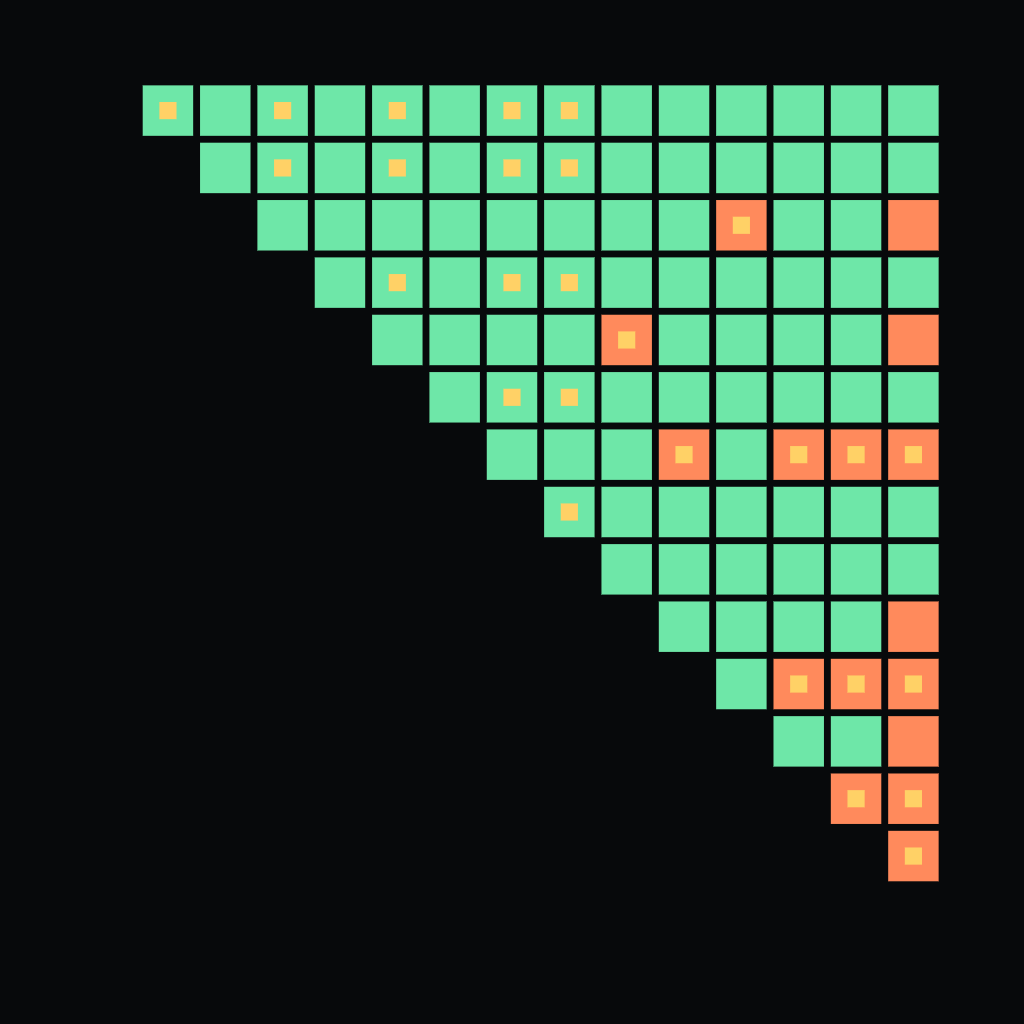
\includegraphics[width=0.5\textwidth]{figures/avatar.png}
\end{center}

\vspace*{\stretch{1.25}}

\newpage

\paperabstract

% BODY
\section{Introduction}
\label{sec:intro}

Take a two-by-two square and colour some of its four cells black. That is a \emph{design}, and there are fifteen nonempty ones. Substitute a shrunken copy of a second design into every black cell of the first, then a third into every black cell of that, and so on. After $L$ steps you have a black-and-white picture on a $2^L \times 2^L$ grid: the Kronecker product $A_{c_1} \otimes \cdots \otimes A_{c_L}$ of the designs you chose, outermost factor first. The list $w = (c_1, \dots, c_L)$ is a \emph{word}, and the picture is its \emph{value}.
\begin{figure}[!ht]
\centering
\witnessplate
\caption{The smallest order-sensitive pair: four black cells either way, four specks one way and two dominoes the other. Every cell is computed by \fpy{}, and the counts are read off the drawing.}
\label{fig:witness}
\end{figure}

The number of black cells does not care about the order of the word. The number of connected black pieces does. \Cref{fig:witness} is the smallest witness: the same two designs, nested both ways, give four separate specks one way and two dominoes the other. That phenomenon, its exact scope at lengths two and three, and a rank-$4$ linear representation of the piece count are the subject of a companion paper \cite{ordersensitivity}; this one starts where that one stops.

Since the order matters at every fixed length, ask about the rate. Fix a two-letter alphabet and an infinite word $w$ over it, write $\comp(A_{w_1 \cdots w_L})$ for the number of $4$-connected black pieces of the length-$L$ prefix, and ask whether
\[
\chi(w) \;=\; \lim_{L \to \infty} \frac{1}{L}\log \comp\bigl(A_{w_1 \cdots w_L}\bigr)
\]
exists, and if it does, whether it can see anything the multiset of letters cannot. The hope, stated plainly so that its refutation is visible: a word like Thue-Morse, aperiodic but with perfectly balanced letter frequencies, ought to return a different number from a periodic word with the same frequencies, and that difference would be a genuinely non-stationary effect in an object whose dimension theory is already known to be a frequency average.

The answer has three parts, and the third one kills the hope.

\medskip
\noindent\textbf{Every alphabet has a closed form.} There is an exact formula for $\comp(A_w)$ on each of the $\binom{15}{2} = 105$ two-letter alphabets, and five regimes, proved from six geometric lemmas, cover them all (\cref{thm:forms}). Two-thirds of the alphabets fall to a single lemma: if either letter has no contact with a copy of itself in either direction, the piece count is the cell count of a prefix, and nothing else needs to be said. The other four regimes are two letters that never break apart, two dominoes at right angles, a run-counting law, and a row-block law.

\medskip
\noindent\textbf{At an interior frequency the rate exists and is order-blind.} If both letters occur with strictly positive frequency, then $\chi(w)$ exists, is a function of the frequency vector alone, and is read off the closed form (\cref{thm:exponent}). Existence is earned from the formula: no ergodic theorem is used, and \cref{prop:norm} says why the matrix-norm route could not supply one. Consequently Thue-Morse returns exactly what a periodic word of the same frequencies returns, and the hoped-for non-stationary effect is not there.

\medskip
\noindent\textbf{And most of the rate is not news.} On $89$ of the $105$ alphabets the rate equals the growth rate of the cell count, which was order-blind to begin with (\cref{thm:saturation}). The one class of alphabets whose rate sits strictly between the constant-word values and that ceiling is a domino against the full tile, where at equal frequencies the rate is $\tfrac12 \log 2$ against per-letter values $0, 0$ and a ceiling of $\tfrac32 \log 2$.

What does fail, cleanly and everywhere, is the obvious guess. A constant word $c^L$ has $\comp(A_{c^L}) = \comp(A_c)^L$, and $\comp(A_c) = 2$ for exactly two of the fifteen designs, so the unique linear functional on the frequency simplex that is exact on constant words is $\Phi(f) = (f_6 + f_9)\log 2$. It is refuted at every interior frequency on $78$ of the $105$ alphabets (\cref{thm:phi}), and changing its coefficients does not repair it: the interior rate is linear, so some linear functional does match it there, but on those alphabets that functional continues to a positive value at a vertex where the constant word has rate $0$, so no continuous frequency functional whatever gives the rate of every word whose letter frequencies and rate both exist. \Cref{fig:ledger} is the whole verdict in one square.

The hypothesis inside every statement above is that both letters occur with positive frequency, and it is not decoration. Over the alphabet $\{3, 6\}$ at the frequency vector $(1,0)$ the constant word has rate $0$, the word carrying the second letter at the square places has rate $\log 2$, and the word carrying it at the powers of $2$ has no rate at all: its prefix rates accumulate on a whole interval (\cref{thm:sharp}). The same three-word pathology occurs on an alphabet carrying no diagonal letter, so it is not a property of one design class.

\subsection*{Where this sits}

Level-varying constructions are not new, and the honest position is that what is owned here is the alphabet and the experiment, not the construction. A word is a non-autonomous iterated function system in the sense of \cite{rempeurbanski}, restricted to a parity-rule alphabet; at similarity maps it is a Moran construction \cite{moran}, and the dimension formulas for varying-ratio constructions \cite{fengwenwu}, specialised to a common base, give the scale dimension of a word as a frequency average. Those are cited, not claimed, and the Feng, Wen and Wu article was unreachable to the author, so its statements are known here only through verbatim restatements in citing papers. In the plane the pictures are generalised Sierpinski carpets in the sense of \cite{cristea2010}, and mixed labyrinth fractals \cite{cristea2017} already own the word \emph{mixed} for level-varying patterns. A randomised schedule is a $V$-variable fractal at $V = 1$ \cite{bhs2008}, whose dimension theory runs through products of random matrices in the companion \cite{bhs2012}. Several distinct ratios inside one level, which this construction cannot express, is the multiscale substitution programme \cite{smilansky}. And a word is an S-adic directive sequence in symbolic dynamics \cite{berthedelecroix}, where the question of which aperiodic words behave well is a mature subject.

What is specific here is narrower. The alphabet is finite, enumerated and classified by symmetry, where the metric-geometric literature takes each level's rule as an arbitrary given subset; the composition law is the Kronecker product, which makes contact multiplicativity one line rather than a graph-directed computation; and order is run as a controlled experiment, holding side, fill, density and dimension fixed while only the letter order moves, which is an experimental design the varying-ratio literature has no reason to run. The scale dimension of a word is a frequency average by the cited formulas, and the point of the component count is that it is the first observable on this construction that is not.

\subsection*{What this paper does not claim}

It does not claim a non-stationary result, and it retires the conjecture that a gap against $\Phi$ would be one. It does not identify $\chi$ for a word whose letter frequencies fail to exist, and \cref{con:nofreq} records the evidence that positive lower density is not the right weaker hypothesis. It says nothing about alphabets of three or more letters, about bases above $2$, about dimensions above $2$, or about the other order-sensitive observables of \cite{ordersensitivity}. It does not decide connectedness: whether a level-varying plane carpet is connected at all, which is the question of whether the count equals $1$, has published necessary and sufficient conditions \cite{cristea2010}, and the formulas here are counts and rates rather than a criterion. The publisher's text of that paper was not reachable to the author either, so its definition, statement and method are known here only through the authors' own companion paper on totally disconnected generalised carpets. No prior art for these counts and rates was found in the literature searched, which is a report on a search and not a claim of novelty.

\section{Definitions}
\label{sec:defs}

\begin{definition}[Designs and codes]
\label{def:design}
A \emph{design} is a subset of the four cells of a $2 \times 2$ grid, encoded by a number $c \in \{1, \dots, 15\}$ whose bit $i$ is the cell at row $\lfloor i/2 \rfloor$ and column $i \bmod 2$. So code $3$ is the top row, code $5$ the left column, code $9$ the main diagonal, code $6$ the antidiagonal, code $7$ the L-shape missing the bottom-right cell, and code $15$ the full tile. Write $A_c \subseteq \{0,1\}^2$ for the set of filled cells and $k_c = |A_c|$ for its \emph{fill}.
\end{definition}

\begin{definition}[Words and their pictures]
\label{def:word}
For a word $w = (c_1, \dots, c_L)$ the picture $A_w \subseteq \{0, \dots, 2^L-1\}^2$ is the Kronecker product $A_{c_1} \otimes \cdots \otimes A_{c_L}$, first letter outermost: a cell with row digits $(r_1, \dots, r_L)$ and column digits $(s_1, \dots, s_L)$ in base $2$ is filled exactly when $(r_i, s_i) \in A_{c_i}$ for every $i$. Its fill is $\fil(A_w) = \prod_i k_{c_i}$, which does not depend on the order. We write $\comp(A_w)$ for the number of $4$-connected components of $A_w$ and $w_{1..i}$ for the prefix of length $i$.
\end{definition}

\begin{definition}[Contacts]
\label{def:contact}
For a picture $X$ of side $n$, $h(X)$ is the number of rows $r$ with both $(r,0)$ and $(r, n-1)$ filled, and $v(X)$ the number of columns $s$ with both $(0,s)$ and $(n-1,s)$ filled. These count the places at which two side-by-side, respectively two stacked, copies of $X$ touch. A design is \emph{contact-free} if $h = v = 0$, which happens exactly for the four one-cell designs $1, 2, 4, 8$ and the two diagonal designs $6, 9$. It is \emph{heavy} if it is connected and $h, v \ge 1$, which happens exactly for the four three-cell designs $7, 11, 13, 14$ and the full tile $15$. The remaining four designs $3, 12, 5, 10$ are the \emph{dominoes}, each with exactly one contact direction; $3$ and $12$ are the row dominoes, $5$ and $10$ the column dominoes; two dominoes are \emph{like} when they share an orientation and \emph{unlike} when they do not.
\end{definition}

The six classes named above, the units $\{1,2,4,8\}$, the row dominoes $\{3,12\}$, the column dominoes $\{5,10\}$, the diagonals $\{6,9\}$, the gaskets $\{7,11,13,14\}$ and the full tile $\{15\}$, are the equivalence classes of every statement in this paper. There are $\binom{15}{2} = 105$ two-letter alphabets and $\binom{6}{2} + 5 = 20$ pairs of classes, of which $15$ pair distinct classes.

\begin{definition}[Frequency and exponent]
\label{def:freq}
An infinite word $w$ over $\{a,b\}$ has \emph{letter frequencies} $f = (f_a, f_b)$ if the number of occurrences of each letter in $w_{1..L}$, divided by $L$, converges. The frequency is \emph{interior} if $f_a > 0$ and $f_b > 0$. The \emph{component exponent} is $\chi(w) = \lim_L \tfrac1L \log\comp(A_{w_{1..L}})$ when the limit exists, and the \emph{fill exponent} is $f_a \log k_a + f_b \log k_b$, which always exists when $f$ does and never depends on the order.
\end{definition}

\begin{definition}[The constant-word functional]
\label{def:phi}
Write $\Phi(f) = (f_6 + f_9)\log 2$. By \cref{lem:constant} below it is the unique linear functional on the frequency simplex that agrees with the rate of every constant word.
\end{definition}

\section{Results}
\label{sec:results}

\subsection{Five regimes close all $105$ alphabets}

\begin{theorem}[The closed forms]
\label{thm:forms}
Let $\{a,b\}$ be one of the $105$ two-letter alphabets and $w$ a word over it of length $L$. Then $\comp(A_w)$ is given exactly by the table below. The first regime is every alphabet with a contact-free letter; the other four assume neither letter is contact-free, so that both are dominoes, gaskets or the full tile, and the five are mutually exclusive and exhaustive.

\medskip
\begin{tabular}{@{}>{\raggedright\arraybackslash}p{0.25\textwidth}>{\raggedright\arraybackslash}p{0.50\textwidth}r@{}}
\toprule
regime & $\comp(A_w)$ & alphabets \\
\midrule
one letter contact-free & $\fil(A_{w_{1..p}})$, with $p$ the last contact-free place, and $1$ if there is none & $69$ \\[2pt]
two heavy letters, or two like dominoes & $1$ & $12$ \\[2pt]
two unlike dominoes & $2^{L-r}$, with $r$ the terminal run & $4$ \\[2pt]
a domino and the full tile & $2^{n-j}$, with $n$ the number of full letters and $j$ their terminal run & $4$ \\[2pt]
a domino and a gasket & $1 + \sum \fil(A_{w_{1..i-1}})$ over the gasket places $i \le m$, with $m$ the last domino place & $16$ \\
\bottomrule
\end{tabular}
\medskip

\noindent In the last row the count is $1$ if $w$ carries no domino. The five counts sum to $105$.
\end{theorem}

The first regime is one lemma, the zero-contact cut, and it settles two-thirds of the table. The proof of the whole theorem is in \cref{sec:proofs}.

\begin{fact}[The forms against the drawing]
\label{fact:forms}
\vpy{} renders $A_w$ cell by cell from \cref{def:word} by an independent route and counts its $4$-connected components by union-find over row runs. On all $26{,}670$ words of length at most $7$ over all $105$ alphabets, and on all $4{,}080$ words of length at most $8$ over the eight named alphabets $(3,7)$, $(5,7)$, $(3,15)$, $(3,6)$, $(3,5)$, $(7,15)$, $(1,3)$, $(6,9)$, the drawn count equals \cref{thm:forms} with zero mismatches.
\end{fact}

\subsection{The exponent at an interior frequency}

\begin{theorem}[Existence, order-blindness, frequency-only]
\label{thm:exponent}
Let $w$ be an infinite word over one of the $105$ alphabets whose letter frequencies exist and are interior. Then $\chi(w)$ exists, depends only on $f$, and equals $f_a \, \epsilon_a + f_b \, \epsilon_b$ with the per-letter weights $\epsilon$ given by the regime:
\begin{itemize}
\item one letter contact-free: $\epsilon_c = \log k_c$ for both letters;
\item two heavy letters, or two like dominoes: $\epsilon_a = \epsilon_b = 0$;
\item two unlike dominoes: $\epsilon_a = \epsilon_b = \log 2$;
\item a domino and the full tile: $\epsilon_{\text{domino}} = 0$ and $\epsilon_{\text{full}} = \log 2$;
\item a domino and a gasket: $\epsilon_{\text{domino}} = \log 2$ and $\epsilon_{\text{gasket}} = \log 3$.
\end{itemize}
In particular $\chi$ is the same along Thue-Morse, along every periodic word with those frequencies, along every strictly ergodic word in which both letters occur, and at almost every Bernoulli word with $0 < p < 1$.
\end{theorem}

\begin{theorem}[Saturation]
\label{thm:saturation}
At every interior frequency the component exponent equals the fill exponent on $89$ of the $105$ alphabets and falls strictly below it on the other $16$. The alphabets on which it falls short are the $12$ of the second regime and the $4$ of the fourth. Among the $16$, exactly the $4$ of the fourth regime, that is a domino against the full tile, have an exponent strictly between $\Phi(f)$ and the fill exponent; at equal frequencies that exponent is $\tfrac12 \log 2$ against per-letter values $0, 0$ and a ceiling of $\tfrac32\log 2$. Up to transposition this is the one class pair with that property.
\end{theorem}

\begin{theorem}[The constant-word functional is refuted]
\label{thm:phi}
At every interior frequency, $\Phi$ is exact on $27$ of the $105$ alphabets and refuted on the other $78$. It is exact exactly on the $15$ alphabets both of whose letters are units or diagonals, and on the $12$ alphabets of the second regime. On each of the $78$ the obstruction sits at a vertex rather than in the interior: changing the coefficients does repair the interior, since the interior formula is itself linear, but the repaired functional extends continuously to the closed simplex and at some vertex takes a positive value while the constant word sitting at that vertex has count $1$ and rate $0$. Hence on those alphabets no continuous functional of $f$ alone gives the rate of every word whose letter frequencies exist and whose rate exists.
\end{theorem}

\begin{figure}[!ht]
\centering
\ledgerplate
\caption{All $105$ two-letter alphabets, indexed by design code along both axes. Lower left triangle: orange where the component exponent meets the fill ceiling ($89$ alphabets), red where it falls short ($16$). Upper right triangle: grey where the constant-word rule $\Phi$ is exact ($27$), blue where it is refuted ($78$). The diagonal is blank, since an alphabet has two distinct letters. Every cell is computed by \fpy{} from the closed forms of \cref{thm:forms}, and the four counts in this caption are printed by the same script.}
\label{fig:ledger}
\end{figure}

\begin{remark}[Two different eighty-nines]
\label{rem:two89}
The $89$ of \cref{thm:saturation} is the set of alphabets whose exponent saturates. There is a second set of size $89$ below, in \cref{cor:smooth}: the alphabets outside the fifth regime, on which every count is $3$-smooth, that is of the form $2^\alpha 3^\beta$. The two are different sets, and since each holds $89$ of the same $105$ they must differ by exactly sixteen on each side. The sixteen of the fifth regime saturate and are not smooth. The sixteen of the second and fourth regimes are smooth and do not saturate: the second because its count is always $1$, and the fourth because its count $2^{n-j}$ is a power of two, while \cref{thm:exponent} gives it the exponent $f_{\text{full}}\log 2$ against a fill exponent of $(1+f_{\text{full}})\log 2$, so it falls short at every interior frequency. The coincidence of size is a coincidence.
\end{remark}

\subsection{Thue-Morse, exactly}

Let $t$ be the Thue-Morse sequence \cite{oeisA010060}, $t_n$ the parity of the binary digit sum of $n$, and read an infinite word over a gasket-and-domino alphabet off it by sending $t_n = 0$ to one letter and $t_n = 1$ to the other, starting at $n = 0$, so that $w_i$ is the letter of $t_{i-1}$. There are two readings, and they give different words.

\begin{theorem}[The Thue-Morse value]
\label{thm:morse}
Over each of the $16$ gasket-and-domino alphabets, and under either reading, the Thue-Morse word has $\chi = \tfrac12 \log 6$, with the two-sided certificate
\[
\Bigl| \log\comp\bigl(A_{w_{1..L}}\bigr) - \tfrac{L}{2}\log 6 \Bigr| \;\le\; \log 108 + \tfrac12 \log\tfrac32 \;<\; 4.885
\]
for every $L \ge 4$.
In nats the value is $0.895879734614027$, and in units of $\log 2$ it is $1.292481250360578$; both are floats naming an exact constant.
\end{theorem}

The certificate does not come from an ergodic theorem or from a fit. It comes from two elementary properties of $t$, that it has no three equal consecutive letters and that its letter counts are exactly balanced, fed into a sandwich bounding $\comp$ between two multiples of one prefix fill. The two alphabets $(3,7)$ and $(5,7)$ are the two whose rate resisted identification longest, and they are covered like the other fourteen.

\begin{fact}[The certificate, measured]
\label{fact:morse}
\vpy{} evaluates the closed form along Thue-Morse under both readings at every length $4 \le L \le 2^{14}$. The largest deviation from $\tfrac{L}{2}\log 6$ is $4.273459$ nats, against the certificate constant $4.884864$. The prefix rate in units of $\log 2$ reads $1.291967463826$ at $L = 4096$ and $1.292352803727$ at $L = 2^{14}$ under one reading, and $1.291291597694$ and $1.292183837194$ under the other, against the limit $1.292481250360578$; all six are floats.
\end{fact}

\begin{fact}[The saturation ratio over one finite sweep]
\label{fact:saturation}
This is the result easiest to overstate: the exponents agree with the fill exponent, and the counts themselves do not. Along Thue-Morse over $(3,7)$ and over $1 \le L \le 2^{14}$, \vpy{} measures the ratio $\comp/\fil$ as taking its smallest value $0.0113766545$, above the floor $1/108$ proved in \cref{lem:sandwich}, and its largest value at $L \ge 5$ as the exact rationals $43397/186624$ under one reading and $151/648$ under the other. The cutoff at $L \ge 5$ is not cosmetic: on the short prefixes \cref{thm:forms} gives the larger values $1/2$ at $L = 1$ and $1/4$ at $L = 4$ in one reading and $1/3$ at $L = 2$ in the other. At $L = 4096$ the ratio is $0.2325367033$, which is neither the largest nor the smallest value of that sweep. Nothing here is a claim about the limit; \cref{con:accum} is what the paper says about that.
\end{fact}

\subsection{Failure modes}

The four statements below are what the investigation refuted, and each was at some point the expected answer. They are stated as results because each of them closes a route.

\begin{remark}[A gap against $\Phi$ is not a non-stationary result]
\label{rem:payoff}
By \cref{thm:exponent}, at an interior frequency $\chi$ is a function of $f$ alone on every one of the $105$ alphabets. So Thue-Morse returns exactly what a periodic word of the same frequencies returns and what almost every Bernoulli word with those frequencies returns, and every one of those stationary words misses $\Phi$ by exactly the same amount. What a gap against $\Phi$ refutes is the frequency functional, not stationarity, and no aperiodic word witnesses anything here. This retires the conjecture that the component exponent is where a level-varying construction stops being a frequency average.
\end{remark}

\begin{theorem}[The interior hypothesis is sharp]
\label{thm:sharp}
Fix the alphabet $\{3,6\}$ and the frequency vector $f = (1,0)$. Then:
\begin{enumerate}
\item the constant word $3^\infty$ has $\chi = 0$;
\item the word carrying the letter $6$ exactly at the square places has $\chi = \log 2$;
\item the word carrying the letter $6$ exactly at the powers of $2$ has upper rate $\log 2$, lower rate $\tfrac12 \log 2$, and no rate, its prefix rates accumulating on the whole interval $[\tfrac12 \log 2, \log 2]$ rather than on its endpoints.
\end{enumerate}
The same three statements hold over the alphabet $\{3,7\}$, which carries no diagonal letter, with the letter $7$ in place of $6$; so the pathology is not a property of the diagonal class. Hence no statement of \cref{thm:exponent} survives dropping the interior hypothesis. The orbit closure of each of the three words is countable and uniquely ergodic, and for the two non-constant words it is not minimal, so no minimal word is implicated. The constant word is of course minimal, and it is the one of the three that does have a rate.
\end{theorem}

\begin{fact}[The boundary rates, measured]
\label{fact:boundary}
For the powers-of-$2$ word over $(3,7)$, \vpy{} reads the prefix rate in units of $\log 2$ as $0.502367981$ at $L = 2048$, $1.002164269$ at $L = 2049$, and $0.500219405$ at $L = 32768$, and over the single block $4097 \le L \le 8192$ it decreases monotonically from $1.00123$ to $0.50073$, which is the interval of \cref{thm:sharp} visible in one sweep. For the same word over $(3,6)$ the prefix rate is exactly $2^k/(2^{k+1}-1)$ at $L = 2^{k+1}-1$, printing $4/7, 8/15, \dots, 8192/16383$, and exactly $1$ at every $L = 2^k$.
\end{fact}

\begin{fact}[The matrix-norm exponent is a different number]
\label{fact:norm}
Restricted to words over $\{3,6\}$ the component count is a rational series of rank $2$: with $\lambda = (1,0)$, $\gamma = (1,1)^{\!\top}$,
\[
M_3 = \begin{pmatrix} 0 & 1 \\ -2 & 3\end{pmatrix}, \qquad M_6 = \begin{pmatrix} 2 & 0 \\ 4 & 0 \end{pmatrix},
\qquad \comp(A_w) = \lambda M_{c_1} \cdots M_{c_L} \gamma ,
\]
verified by \vpy{} on all $8{,}190$ words of length at most $12$, and the largest entry of $M_3^L$ is $2^{L+1}-1$ at every $L \le 24$.
\end{fact}

\begin{proposition}[The matrix-norm exponent is a different number]
\label{prop:norm}
$\lim_L \tfrac1L \log \lVert M_3^L \rVert = \log 2$ in any matrix norm, while $\chi(3^\infty) = 0$. Hence no argument that returns a top Lyapunov exponent \cite{furstenbergkesten} or a joint spectral radius \cite{jungers}, and no projective-contraction argument on forward orbits, can return $\chi$: they answer a different question. The rank-$4$ representation over the full alphabet, and the invariant cone it carries, belong to \cite{ordersensitivity}; neither is used anywhere in this paper, and this proposition is why neither would help.
\end{proposition}

\begin{proof}
$M_3$ has characteristic polynomial $\lambda^2 - 3\lambda + 2$, so its eigenvalues are $1$ and $2$ and its spectral radius is $2$; by Gelfand's formula the norm exponent is $\log 2$. Explicitly, splitting $M_3$ over its eigenvectors gives
\[
M_3^L = \begin{pmatrix} 2 - 2^L & 2^L - 1 \\ 2 - 2^{L+1} & 2^{L+1} - 1\end{pmatrix},
\]
whose largest entry in absolute value is $2^{L+1}-1$, which is the number \cref{fact:norm} measures. On the other side $\comp(A_{3^L}) = 1$ at every $L$ by \cref{lem:constant}, so $\chi(3^\infty) = 0$.
\end{proof}

\begin{remark}[Thue-Morse is not a non-existence witness]
\label{rem:notmorse}
A headline that does not exist, said out loud so that it is not written later: the component exponent does not fail to exist along Thue-Morse. It converges, exactly, by \cref{thm:morse}. The genuine non-existence witness is the third word of \cref{thm:sharp}, which sits at a boundary frequency and whose orbit closure is not minimal.
\end{remark}

\subsection{What stays open}

\begin{conjecture}[Words with no letter frequencies]
\label{con:nofreq}
Positive lower density of both letters is not enough for $\chi$ to exist. Over $(3,7)$ the tripling word $W_{k+1} = W_k \, 7^{|W_k|} 3^{|W_k|}$ with $W_1 = (7,3)$ keeps both letters at lower density at least $1/4$, and \vpy{} finds its prefix rate ranging over $[0.4792, 1.4379]$ in units of $\log 2$ on $1024 \le L \le 4096$ with no narrowing. The closed form is exact there; the non-existence of the limit is measurement, not proof. Which words without letter frequencies carry a component exponent is open.
\end{conjecture}

\begin{conjecture}[The accumulation set of the saturation]
\label{con:accum}
Whether $\comp/\fil$ converges at all along Thue-Morse over a gasket-and-domino alphabet is open, and the measurement of \cref{fact:saturation} is that it does not settle over $1 \le L \le 2^{14}$, its values there spreading over more than a factor of twenty. Its accumulation set is unidentified, and is plausibly the attractor of the two affine maps that the two letters induce on the normalised chart. \Cref{lem:sandwich} traps every value at $L \ge 4$ in $(1/108, 5/12]$.
\end{conjecture}

\begin{conjecture}[Where a non-stationary effect could still live]
\label{con:three}
Nothing here speaks about alphabets of three or more letters, about the Euler characteristic, boundary or hole counts, whose representations have larger rank \cite{ordersensitivity}, or about bases above $2$. Whether any of them makes the exponent depend on more than the letter frequencies, which is what a genuinely non-stationary result would need, is open; at an interior frequency on two letters it provably does not.
\end{conjecture}

\section{Proofs}
\label{sec:proofs}

\subsection{Six lemmas}

\begin{lemma}[Contacts multiply]
\label{lem:contact}
$h(A_w) = \prod_i h(A_{c_i})$ and $v(A_w) = \prod_i v(A_{c_i})$.
\end{lemma}

\begin{proof}
It suffices to treat $A \otimes B$ with $A$ of side $m$ and $B$ of side $n$. A row of $A \otimes B$ is indexed by a pair $(r, r')$ with $r < m$, $r' < n$, and its first and last cells are $(r,r')$-indexed cells of the leftmost and rightmost blocks, that is the cells $(r', 0)$ of $B$ inside block column $0$ of $A$ and $(r', n-1)$ of $B$ inside block column $m-1$. So row $(r,r')$ of $A \otimes B$ has both end cells filled exactly when row $r$ of $A$ has both end cells filled and row $r'$ of $B$ has both end cells filled. Counting pairs gives $h(A \otimes B) = h(A)h(B)$, and the column statement is the transpose. Induction on the length finishes it.
\end{proof}

\begin{lemma}[The zero-contact cut]
\label{lem:cut}
\emph{(a)} If $h(A_u) = v(A_u) = 0$ for a suffix $u = w_{p..L}$, then $\comp(A_w) = \fil(A_{w_{1..p-1}}) \cdot \comp(A_u)$. \emph{(b)} If $z$ is contact-free then $\comp(A_{zu}) = k_z \cdot \comp(A_u)$ for every word $u$, and in particular $\comp(A_z) = k_z$.
\end{lemma}

\begin{proof}
For (a), write $A_w = A_{w_{1..p-1}} \otimes A_u$. Each filled cell of $A_{w_{1..p-1}}$ carries one translated copy of $A_u$ inside its own block, and two cells of $A_w$ lying in different blocks are $4$-adjacent only if the two blocks sit at $4$-adjacent cells of $A_{w_{1..p-1}}$, since two distinct block row-ranges overlap only when the block rows agree, and likewise for columns. Two blocks at horizontally adjacent cells contribute a $4$-adjacent pair exactly when some row of $A_u$ has both its end cells filled, that is when $h(A_u) \ge 1$; vertically adjacent blocks likewise need $v(A_u) \ge 1$. Both are zero, so distinct copies never merge, and the component count is the number of copies times the component count of one copy.

For (b), a contact-free design is either a single cell or one of the two diagonal designs, so its filled cells are pairwise non-$4$-adjacent. Hence in $A_z \otimes A_u$ the $k_z$ copies of $A_u$ sit in pairwise non-adjacent blocks and never touch, whatever the contacts of $A_u$.
\end{proof}

\begin{lemma}[A heavy suffix letter does nothing]
\label{lem:heavy}
If $c$ is heavy then $\comp(A_{wc}) = \comp(A_w)$ for every word $w$.
\end{lemma}

\begin{proof}
In $A_w \otimes A_c$ each filled cell of $A_w$ becomes a block congruent to $A_c$, which is connected. Two blocks at horizontally adjacent cells meet exactly when $h(A_c) \ge 1$, two at vertically adjacent cells exactly when $v(A_c) \ge 1$, and both hold; two blocks at non-adjacent cells are disjoint and never touch. So the graph on blocks with an edge when two blocks meet is isomorphic to the graph on filled cells of $A_w$ with an edge when two cells are $4$-adjacent, and connected components correspond. The base case $\comp(A_c) = 1$ is connectedness of $A_c$.
\end{proof}

\begin{lemma}[A domino suffix letter counts runs]
\label{lem:runs}
Let $H(X)$ be the number of maximal horizontal runs of filled cells of $X$, summed over rows. For a row domino $p$, $\comp(A_{wp}) = H(A_w)$. Moreover $H(\varepsilon) = 1$, $H(A_{wp}) = H(A_w)$ at a row domino $p$, and $H(A_{wq}) = H(A_w) + \fil(A_w)$ at a gasket $q$. The transposed statements hold for column dominoes with vertical runs.
\end{lemma}

\begin{proof}
A row domino has one full row and one empty row. In $A_w \otimes A_p$ every filled cell of $A_w$ becomes a block whose one filled row is the same row of the block for every block, and the other row of each block is empty. Rows of $A_w \otimes A_p$ therefore alternate between a copy of a row of $A_w$ with each cell doubled and an empty row, so no two filled rows are vertically adjacent, and doubling each cell merges exactly the cells that were already horizontally adjacent. Hence components are in bijection with maximal horizontal runs of $A_w$, which is the first claim, and the run count is unchanged, which is the second.

For a gasket $q$: each of $7, 11, 13, 14$ has one full row and one row with a single cell. In $A_w \otimes A_q$ the rows carrying the full row of each block reproduce the runs of $A_w$ with each cell doubled, giving $H(A_w)$ runs; the rows carrying the one-cell row of each block hold one isolated cell per filled cell of $A_w$, since consecutive blocks are two columns apart and the single cells occupy the same column of each block, giving $\fil(A_w)$ runs. Adding gives $H(A_{wq}) = H(A_w) + \fil(A_w)$.
\end{proof}

\begin{lemma}[The row-block law]
\label{lem:block}
Over an alphabet consisting of one row domino and the full tile, $\comp(A_w) = 2^{n-j}$ with $n$ the number of full letters in $w$ and $j$ the length of the terminal run of full letters. The transposed statement holds for a column domino.
\end{lemma}

\begin{proof}
A row domino forces the row digit at its place, say to the value $d$, and leaves the column digit free; the full tile forces neither. So the filled set is a product $R \times \{0, \dots, 2^L-1\}$, where $R$ is the set of rows whose digit equals $d$ at every domino place, and $|R| = 2^n$. Every row of $R$ is a full horizontal line, so two of them lie in the same component exactly when they are vertically adjacent, and the component count is the number of maximal blocks of consecutive integers in $R$.

Index the row digits so that place $i$ contributes $2^{L-i}$. The last $j$ places are full, hence free, and place $L-j$ is a domino, hence forced, whenever $j < L$. So $R$ is a union of blocks of $2^j$ consecutive integers, one for each choice of the free digits above place $L-j$, and the integer just above such a block differs from its top element by flipping the forced digit at place $L-j$ from $d$, so it is not in $R$ and the blocks are pairwise non-adjacent. There are $2^{n-j}$ of them. If $j = L$ then $R$ is everything and the count is $1 = 2^{n-j}$; if $n = 0$ then $j = 0$, $R$ is a single row and the count is $1$.
\end{proof}

\begin{lemma}[Constant words]
\label{lem:constant}
$\comp(A_{c^L}) = \comp(A_c)^L$ for every code $c$, and $\comp(A_c) = 2$ exactly for $c \in \{6,9\}$ and $1$ for the other thirteen.
\end{lemma}

\begin{proof}
A unit design has fill $1$, so $A_{c^L}$ is one cell. A domino word of one orientation is a full line, hence connected, by \cref{lem:runs} applied repeatedly or directly: the filled set is a product of a single forced row with the whole column range. A heavy letter gives $1$ at every length by \cref{lem:heavy}. A diagonal letter is contact-free with fill $2$, so \cref{lem:cut} applies at every suffix and $\comp(A_{c^L}) = 2^L$. Finally $\comp(A_c)$ is $1$ for the nine designs of fill $1, 3, 4$ and for the four dominoes, and $2$ for the two diagonals, since the two cells of a diagonal design are not $4$-adjacent.
\end{proof}

\subsection{Proof of \texorpdfstring{\cref{thm:forms}}{the closed forms}}

\begin{proof}
The five regimes are mutually exclusive and exhaust the $105$ alphabets. Counting: the contact-free designs are the six codes $1,2,4,8,6,9$, so the alphabets meeting the first regime number $\binom{6}{2} + 6 \cdot 9 = 15 + 54 = 69$. The remaining $\binom{9}{2} = 36$ alphabets lie among the four dominoes, the four gaskets and the full tile, and split as $10$ pairs of heavy letters plus $2$ pairs of like dominoes, giving $12$; $4$ pairs of unlike dominoes; $4$ pairs of a domino with the full tile; and $4 \cdot 4 = 16$ pairs of a domino with a gasket. Then $69 + 12 + 4 + 4 + 16 = 105$.

\emph{First regime.} Suppose first that both letters are contact-free. Then $p = L$, and the one-letter suffix $w_L$ has zero contact, so \cref{lem:cut}(a) followed by \cref{lem:cut}(b) gives
\[
\comp(A_w) = \fil\bigl(A_{w_{1..L-1}}\bigr) \comp\bigl(A_{w_L}\bigr) = \fil\bigl(A_{w_{1..L-1}}\bigr) k_{w_L} = \fil\bigl(A_{w_{1..p}}\bigr).
\]

Otherwise exactly one letter $z$ is contact-free; call the other $c$. If $w$ carries no $z$ then $w = c^L$ with $c$ a domino, a gasket or the full tile, so $\comp(A_w) = 1$ by \cref{lem:constant}, which is the stated value. Otherwise let $p$ be the last place carrying $z$. Every letter after $p$ equals $c$, so the suffix $u = w_{p..L} = z\,c^{L-p}$ has $h(A_u) = h(A_z) h(A_c)^{L-p} = 0$ and likewise $v(A_u) = 0$ by \cref{lem:contact}. Then \cref{lem:cut}(a) gives $\comp(A_w) = \fil(A_{w_{1..p-1}}) \comp(A_u)$, and \cref{lem:cut}(b) applied to $u$ gives $\comp(A_u) = k_z \comp(A_{c^{L-p}}) = k_z$, using $\comp(A_{c^{L-p}}) = 1$ from \cref{lem:constant}. Multiplying, $\comp(A_w) = \fil(A_{w_{1..p-1}}) k_z = \fil(A_{w_{1..p}})$.

\emph{Second regime.} If both letters are heavy then $\comp(A_w) = 1$ by \cref{lem:heavy} and induction on the length. If both are row dominoes then every letter forces the row digit at its place and leaves the column digit free, so the filled set is a single full row; if both are column dominoes the transposed argument gives a single full column. Either way $\comp(A_w) = 1$.

\emph{Third regime.} Let $r$ be the length of the terminal run and suppose first $r < L$, so that place $L-r$ carries the other orientation. The suffix $u = w_{L-r..L}$ satisfies $h(A_u) = h(A_{w_{L-r}}) h(A_{w_L})^{r}$ and $v(A_u) = v(A_{w_{L-r}}) v(A_{w_L})^{r}$; one of the two orientations has $h = 0$ and the other has $v = 0$, so both products vanish. \Cref{lem:cut} gives $\comp(A_w) = \fil(A_{w_{1..L-r-1}}) \comp(A_u) = 2^{L-r-1}\comp(A_u)$. And $\comp(A_u) = 2$, computed directly: up to transposition $A_u$ is a column domino carrying in each of its two cells a copy of $A_{w_L^{\,r}}$, which is a full horizontal line at one row of its $2^r \times 2^r$ block; the two copies occupy blocks one above the other, so the two lines sit $2^r \ge 2$ rows apart and are not adjacent. Hence $\comp(A_w) = 2^{L-r}$. If $r = L$ the word is constant, $\comp(A_w) = 1 = 2^{L-r}$.

\emph{Fourth regime.} This is \cref{lem:block}.

\emph{Fifth regime.} Let $q$ be the gasket and $p$ the domino, and suppose without loss of generality that $p$ is a row domino, the column case being the transpose. If $w$ carries no domino then $w = q^L$ and $\comp(A_w) = 1$ by \cref{lem:heavy}. Otherwise let $m$ be the last domino place. Every letter after $m$ is the gasket, which is heavy, so $\comp(A_w) = \comp(A_{w_{1..m}})$ by \cref{lem:heavy}. The last letter of $w_{1..m}$ is the row domino, so $\comp(A_{w_{1..m}}) = H(A_{w_{1..m-1}})$ by \cref{lem:runs}. Finally the run recursion of \cref{lem:runs} telescopes: starting from $H(\varepsilon) = 1$ and reading $w_{1..m-1}$ letter by letter, each domino leaves $H$ unchanged and each gasket at place $i$ adds $\fil(A_{w_{1..i-1}})$. Hence $H(A_{w_{1..m-1}}) = 1 + \sum \fil(A_{w_{1..i-1}})$ over gasket places $i \le m-1$, and since $m$ itself is a domino place this is the sum over gasket places $i \le m$.
\end{proof}

\subsection{Proof of \texorpdfstring{\cref{thm:exponent}}{the exponent theorem}}

\begin{lemma}[Terminal runs vanish at interior frequency]
\label{lem:terminal}
Let $w$ be an infinite word over $\{a,b\}$ whose letter frequencies exist and are interior, and let $r(L)$ be the length of the terminal run of $w_{1..L}$. Then $r(L) = o(L)$.
\end{lemma}

\begin{proof}
Suppose not, so there are $\varepsilon > 0$ and lengths $L_1 < L_2 < \cdots$ with $r(L_i) \ge \varepsilon L_i$. Let $x$ be a letter not equal to the repeated letter of the run at $L_i$, passing to a subsequence so that $x$ is the same letter throughout, and let $N_x(L)$ count occurrences of $x$ in $w_{1..L}$. Then $N_x(L_i) = N_x(L_i - r(L_i))$, since $x$ does not occur in the terminal run. Set $M_i = L_i - r(L_i) \le (1-\varepsilon) L_i$. If $M_i$ is bounded then $N_x(L_i)$ is bounded and $f_x = 0$. Otherwise $N_x(M_i)/M_i \to f_x$, so
\[
\frac{N_x(L_i)}{L_i} = \frac{N_x(M_i)}{M_i}\cdot\frac{M_i}{L_i} \le \bigl(f_x + o(1)\bigr)(1-\varepsilon),
\]
while the left side tends to $f_x$. Hence $f_x \le (1-\varepsilon) f_x$, so $f_x = 0$, contradicting interiority.
\end{proof}

\begin{proof}[Proof of \cref{thm:exponent}]
Write $N_c(L)$ for the count of the letter $c$ in $w_{1..L}$, so $N_c(L)/L \to f_c$.

\emph{First regime.} By \cref{thm:forms}, $\log\comp(A_{w_{1..L}}) = \log\fil(A_{w_{1..p(L)}})$ with $p(L)$ the last contact-free place. If both letters are contact-free then $p(L) = L$ and the right side is $\sum_{i \le L} \log k_{w_i}$, whose average tends to $f_a \log k_a + f_b \log k_b$. Otherwise $L - p(L)$ is the terminal run of the non-contact-free letter, hence $o(L)$ by \cref{lem:terminal}, and
\[
\log \fil\bigl(A_{w_{1..p(L)}}\bigr) = \log\fil\bigl(A_{w_{1..L}}\bigr) - \bigl(L - p(L)\bigr)\log k_c = \sum_{i\le L} \log k_{w_i} + o(L),
\]
giving the same limit. Both cases are the fill exponent, which is the stated weight table since $\epsilon_c = \log k_c$.

\emph{Second regime.} $\comp \equiv 1$, so $\chi = 0$.

\emph{Third regime.} $\log\comp = (L - r(L))\log 2 = L\log 2 + o(L)$ by \cref{lem:terminal}.

\emph{Fourth regime.} $\log\comp = (n(L) - j(L))\log 2$ with $n(L)$ the number of full letters, so $n(L)/L \to f_{\text{full}}$, and $j(L)$ a terminal run, hence $o(L)$ by \cref{lem:terminal}. The limit is $f_{\text{full}}\log 2$.

\emph{Fifth regime.} Let $m(L)$ be the last domino place and $i^*(L)$ the last gasket place at or before $m(L)$; both exist for large $L$ because both frequencies are positive. Then $L - m(L)$ is a terminal run of gaskets, hence $o(L)$, and $m(L) - i^*(L)$ is the terminal run of $w_{1..m(L)}$, hence $o(m(L)) = o(L)$, both by \cref{lem:terminal}. Write $T(L) = \fil(A_{w_{1..i^*(L)-1}})$. By \cref{lem:sandwich} below, $T(L) < \comp(A_{w_{1..L}}) \le 1 + \tfrac32 T(L)$, so $\log\comp = \log T(L) + O(1)$. And
\begin{align*}
\log T(L) &= \sum_{i < i^*(L)} \log k_{w_i} = \sum_{i \le L} \log k_{w_i} - O\bigl(L - i^*(L)\bigr) \\
&= L\bigl(f_p \log 2 + f_q \log 3\bigr) + o(L),
\end{align*}

since $L - i^*(L) = o(L)$ and each $\log k_{w_i} \le \log 3$. Dividing by $L$ gives the claim.

In all five cases the limit is a function of $f$ alone. The final sentence follows: Thue-Morse, every periodic word, and every strictly ergodic word carrying both letters have letter frequencies, interior in the last two cases by minimality and in the first because both letters have frequency $\tfrac12$; and a Bernoulli word has frequencies $(p, 1-p)$ almost surely by the strong law.
\end{proof}

\begin{lemma}[The sandwich]
\label{lem:sandwich}
Over a gasket-and-domino alphabet, let $m$ be the last domino place of $w$, let $i^*$ be the last gasket place at or before $m$, and put $T = \fil(A_{w_{1..i^*-1}})$. Then $T < \comp(A_w) \le 1 + \tfrac32 T$. Moreover $\fil(A_w)/T \in [6, 108]$ whenever no three consecutive letters of $w$ are equal, and then $\comp(A_w)/\fil(A_w) \in (1/108,\, 5/12]$, with no side condition, since $T \ge 1$ always.
\end{lemma}

\begin{proof}
By \cref{thm:forms}, $\comp(A_w) = 1 + \sum_i \fil(A_{w_{1..i-1}})$ over gasket places $i \le m$. The largest term is the one at $i = i^*$, namely $T$, so $\comp(A_w) > T$. If $i < i'$ are two consecutive gasket places at or before $m$ then $\fil(A_{w_{1..i'-1}})/\fil(A_{w_{1..i-1}}) = \fil(A_{w_{i..i'-1}}) \ge k_q = 3$, since $w_i$ is a gasket and the other letters of the block have fill at least $2$. Reading the terms backwards from $T$ they therefore decrease by factors of at least $3$, so their sum is at most $T(1 + \tfrac13 + \tfrac19 + \cdots) = \tfrac32 T$, giving $\comp(A_w) \le 1 + \tfrac32 T$.

For the second claim, the suffix $w_{i^*..L}$ has the shape $q\, p^{\,\alpha}\, q^{\,\beta}$ with $\alpha = m - i^* \ge 1$ and $\beta = L - m \ge 0$, because $i^*$ is the last gasket place at or before $m$ and $m$ is the last domino place. So $\fil(A_w)/T = 3 \cdot 2^{\alpha} 3^{\beta}$. If no three consecutive letters agree then $\alpha \le 2$ and $\beta \le 2$, so this lies in $[3 \cdot 2, \, 3 \cdot 4 \cdot 9] = [6, 108]$. Finally $1 + \tfrac32 T \le \tfrac52 T$ as soon as $T \ge 1$, which holds for every word since a fill is at least $1$, so $\comp \le \tfrac52 T$, so $\comp/\fil \le (\tfrac52 T)/(6T) = \tfrac{5}{12}$, and $\comp/\fil > T/(108\,T) = 1/108$.
\end{proof}

\subsection{Proof of \texorpdfstring{\cref{thm:saturation,thm:phi}}{the two counting theorems}}

\begin{proof}
Both are a walk through the five regimes with the weights of \cref{thm:exponent} in hand. Write $\phi_c = \log 2$ if $c$ is a diagonal and $0$ otherwise, so that $\Phi(f) = f_a \phi_a + f_b \phi_b$, and write $\epsilon_c$ for the exponent weight and $\log k_c$ for the fill weight. Since one frequency is free on the open simplex, $\chi$ equals the fill exponent at every interior $f$ if and only if $\epsilon_c = \log k_c$ for both letters, and $\Phi$ is exact at every interior $f$ if and only if $\epsilon_c = \phi_c$ for both letters.

\emph{First regime, $69$ alphabets.} $\epsilon_c = \log k_c$ for both letters, so all $69$ saturate. And $\epsilon_c = \phi_c$ requires $\log k_c = \phi_c$ for each letter, which holds for a unit ($k = 1$, $\phi = 0$) and a diagonal ($k = 2$, $\phi = \log 2$) and fails for a domino ($k = 2$, $\phi = 0$), a gasket ($k = 3$) and the full tile ($k = 4$). So $\Phi$ is exact on the $\binom{6}{2} = 15$ alphabets both of whose letters are units or diagonals and refuted on the other $54$.

\emph{Second regime, $12$ alphabets.} $\epsilon_a = \epsilon_b = 0$; the letters are dominoes, gaskets or the full tile, all of fill at least $2$, so saturation fails on all $12$. No letter is a diagonal, so $\phi_a = \phi_b = 0$ and $\Phi$ is exact on all $12$.

\emph{Third regime, $4$ alphabets.} $\epsilon = \log 2 = \log k$ for both letters, so all $4$ saturate; $\phi = 0 \ne \log 2$, so $\Phi$ is refuted on all $4$.

\emph{Fourth regime, $4$ alphabets.} $\epsilon_{\text{domino}} = 0 \ne \log 2 = \log k_{\text{domino}}$, so none saturates; $\epsilon_{\text{full}} = \log 2 \ne 0 = \phi_{\text{full}}$, so $\Phi$ is refuted on all $4$.

\emph{Fifth regime, $16$ alphabets.} $\epsilon = \log k$ for both letters, so all $16$ saturate; $\phi = 0$ for both while $\epsilon \ne 0$, so $\Phi$ is refuted on all $16$.

Adding, saturation holds on $69 + 4 + 16 = 89$ and fails on $12 + 4 = 16$; $\Phi$ is exact on $15 + 12 = 27$ and refuted on $54 + 4 + 4 + 16 = 78$.

For the strictly-between claim, an alphabet has $\Phi(f) < \chi(f) < $ fill exponent at interior $f$ exactly when saturation fails and $\Phi$ is refuted, since otherwise one of the two inequalities is an equality. Saturation fails only in the second and fourth regimes, and $\Phi$ is exact throughout the second, so only the fourth regime survives: the $4$ alphabets of a domino against the full tile, one class pair up to transposition. At $f = (\tfrac12,\tfrac12)$ its exponent is $\tfrac12 \log 2$, against $\Phi = 0$ and a fill exponent of $\tfrac12\log 2 + \tfrac12 \log 4 = \tfrac32 \log 2$.

Finally the wrong-shape statement of \cref{thm:phi}. On each of the $78$, pick a vertex of the simplex at which the interior formula reads a positive value. In the first regime with a refuting letter $c$ the interior formula is the fill exponent, which reads $\log k_c > 0$ at the vertex $f = \delta_c$ for any letter of fill at least $2$; in the third it reads $\log 2$ at both vertices; in the fourth it reads $\log 2$ at the full-tile vertex; in the fifth it reads $\log 2$ or $\log 3$ at the two vertices. The constant word at that vertex has rate $0$, since its letter is not a diagonal in any of the cases listed. A continuous functional agreeing with $\chi$ in the interior takes the interior formula's value at that vertex by continuity, which is positive, so it misses the constant word.
\end{proof}

\subsection{Proof of \texorpdfstring{\cref{thm:morse}}{the Thue-Morse value}}

\begin{proof}
Two properties of the Thue-Morse sequence do all the work. First, no three consecutive terms are equal: among any three consecutive indices there is an even index $2n$ whose successor $2n+1$ is also among them, and $t_{2n} = t_n$ while $t_{2n+1} = 1 - t_n$, so those two differ. Second, the letter counts are exactly balanced: the prefix $w_{1..L}$ reads the indices $0, \dots, L-1$, and pairing them as $(2k, 2k+1)$ each pair contributes one of each letter, so a prefix of even length $L$ has exactly $L/2$ of each and a prefix of odd length has $\lfloor L/2 \rfloor$ or $\lceil L/2 \rceil$; in both cases $|N_q(L) - L/2| \le \tfrac12$.

Fix a gasket-and-domino alphabet, a reading, and $L \ge 4$, which is what it takes for a gasket place and a domino place both to occur, so that $m$ and $i^*$ are defined. No lower bound on $T$ is needed, and none is available: under the reading sending $0$ to the gasket the prefix of length $4$ is $q\,p\,p\,q$, whose $i^*$ is $1$ and whose $T$ is therefore $\fil(A_\varepsilon) = 1$. By \cref{lem:sandwich} and the first property, $\comp(A_{w_{1..L}})/\fil(A_{w_{1..L}}) \in (1/108, 5/12]$, hence
\[
\Bigl|\log\comp\bigl(A_{w_{1..L}}\bigr) - \log \fil\bigl(A_{w_{1..L}}\bigr)\Bigr| \le \log 108 .
\]
By the second property, with $N_q$ the gasket count and $N_p = L - N_q$ the domino count,
\begin{align*}
\Bigl|\log\fil\bigl(A_{w_{1..L}}\bigr) - \tfrac{L}{2}\log 6\Bigr|
&= \Bigl| \bigl(N_p - \tfrac{L}{2}\bigr)\log 2 + \bigl(N_q - \tfrac{L}{2}\bigr)\log 3\Bigr| \\
&= \Bigl|N_q - \tfrac{L}{2}\Bigr| \log\tfrac32 \;\le\; \tfrac12 \log\tfrac32 ,
\end{align*}
using $N_p - \tfrac L2 = -(N_q - \tfrac L2)$. Adding the two displays gives the certificate, and $\log 108 + \tfrac12\log\tfrac32 = 4.884864\ldots < 4.885$. Dividing by $L$ and letting $L \to \infty$ gives $\chi = \tfrac12 \log 6$. Nothing in the argument names the alphabet beyond the fills $3$ and $2$, so it covers all $16$ alphabets and both readings.
\end{proof}

\subsection{Proof of \texorpdfstring{\cref{thm:sharp}}{sharpness}}

\begin{proof}
Over $\{3,6\}$ the letter $6$ is contact-free and the letter $3$ is not, so the first regime of \cref{thm:forms} applies and $\comp(A_{w_{1..L}}) = \fil(A_{w_{1..p(L)}}) = 2^{p(L)}$ with $p(L)$ the last place of $w_{1..L}$ carrying the letter $6$, both letters having fill $2$. In each of the three words the letter $6$ occurs on a set of density $0$, so $f = (1,0)$.

For the constant word $p(L) = 0$ and $\comp \equiv 1$, so $\chi = 0$. For the squares word $p(L) = \lfloor \sqrt L\rfloor^2$, and $\lfloor\sqrt L\rfloor^2/L \to 1$, since for $L$ in $[n^2, (n+1)^2)$ the ratio is at least $n^2/((n+1)^2-1) \to 1$, so $\chi = \log 2$. For the powers-of-$2$ word $p(L) = 2^{\lfloor \log_2 L\rfloor}$, so the prefix rate in units of $\log 2$ is $2^k/L$ for $L \in [2^k, 2^{k+1})$, which equals $1$ at $L = 2^k$ and decreases to just above $\tfrac12$ at $L = 2^{k+1}-1$, in steps of size at most $2^k/L - 2^k/(L+1) \le 1/L$. Every point of $[\tfrac12, 1]$ is therefore within $1/L$ of a value taken in the $k$-th block, so the accumulation set of the prefix rates is exactly $[\tfrac12, 1]$ in units of $\log 2$, the upper rate is $\log 2$, the lower rate is $\tfrac12\log 2$, and the limit does not exist.

Over $\{3,7\}$ the fifth regime applies. For the word carrying $7$ exactly at the powers of $2$ and $L$ in $(2^k, 2^{k+1}]$, the last domino place $m$ is $L$ unless $L$ is a power of $2$, in which case it is $L - 1$; in either case the last gasket place at or before $m$ is $i^* = 2^k$ for $L > 2^k$. So $T = \fil(A_{w_{1..2^k-1}}) = 2^{2^k-1-k}3^{k}$ and \cref{lem:sandwich} gives $\log_2 \comp = 2^k + O(k)$ throughout the block. The prefix rate is therefore $2^k/L + O(k/L)$, and the argument of the previous paragraph applies verbatim. The constant word $3^\infty$ has $\comp \equiv 1$ by \cref{thm:forms} with no domino-free reading needed, and the squares word has $\log_2\comp = \lfloor\sqrt L\rfloor^2 + O(\sqrt L)$ by the same sandwich, hence rate $\log 2$. All three words have $f = (1,0)$.

Each of the three orbit closures is the closure of the shift orbit of a word whose non-constant letters have density $0$, hence countable, with the point mass at the constant word as its only shift-invariant measure, so all three are uniquely ergodic. For the two non-constant words the closure properly contains the fixed point of the shift and so is not minimal; the first word is the constant word itself, whose orbit closure is a single point and is minimal.
\end{proof}

\begin{fact}[A stationary control, and the one rough family]
\label{fact:byproduct}
$\comp(A_{(7,3)^k}) = (6^k+4)/5$, reading $2$, $8$, $44$, $260$, $1556$, $9332$, checked by \vpy{} to $k = 8$ against \cref{thm:forms} and to $k = 4$ against the drawing. Its per-letter rate is $\tfrac12\log 6$ again, from a periodic and therefore stationary word. And the fifth regime really does leave the smooth numbers of \cref{cor:smooth} behind: the largest count at length $8$ over the alphabet $(3,7)$ is $1094 = 2 \cdot 547$, checked by \vpy{} over all words of that length.
\end{fact}

\begin{corollary}[Every count off the fifth regime is $3$-smooth]
\label{cor:smooth}
On each of the $89$ alphabets outside the fifth regime, every count $\comp(A_w)$ has the form $2^\alpha 3^\beta$. A gasket against a domino is therefore the only family whose counts need a prime above $3$.
\end{corollary}

\begin{proof}
Read \cref{thm:forms} regime by regime. In the first the count is $\fil(A_{w_{1..p}})$, a product of fills drawn from $\{1,2,3,4\}$, hence of the form $2^\alpha 3^\beta$; in the second it is $1$; in the third it is $2^{L-r}$; in the fourth it is $2^{n-j}$. Only the fifth regime produces a sum rather than a product, and only there can another prime appear.
\end{proof}

\begin{remark}[Words are not recoverable from pictures]
\label{rem:monoid}
Nothing above tries to read the word off the picture, and it could not: Kronecker factorisation of a binary matrix is unique at a fixed profile of factor sizes but not once the profile may vary, and a matrix can factor at profiles of different length and at factor sizes that are not prime. That is settled in \cite{voet}, and it is why the object of study here is the alphabet and the word, not the tile.
\end{remark}

\section{Reproducibility}
\label{sec:repro}

Two scripts, both plain \texttt{python3} with nothing beyond the standard library, both run from the paper's directory, both using relative paths only.

\texttt{python3 scripts/verify.py} runs in about $15$ seconds on a laptop and dies loudly, naming the word and both values, at the first disagreement. It checks:

\begin{itemize}
\item \emph{Contacts multiply.} All $54{,}240$ words of length $1$ to $4$ over the $15$ codes: $h$ and $v$ of the drawn picture against the product of the per-letter values (\cref{lem:contact}).
\item \emph{The regime census.} That the five regimes partition the $105$ alphabets as $69, 12, 4, 4, 16$ (\cref{thm:forms}).
\item \emph{The closed forms against the drawing.} All $26{,}670$ words of length at most $7$ over all $105$ alphabets, and all $4{,}080$ words of length at most $8$ over eight named alphabets, drawn cell by cell and counted by union-find over row runs (\cref{fact:forms}).
\item \emph{The rate table.} For each of the $105$ alphabets, the prefix rate of the closed form at length $4000$, at two different letter frequencies, against $f_a\epsilon_a + f_b\epsilon_b$ from \cref{thm:exponent}, to within $0.02$.
\item \emph{The verdict counts.} The counts $89$ and $16$ of \cref{thm:saturation}, $27$ and $78$ of \cref{thm:phi}, and that exactly $4$ alphabets are strictly between and all four are a domino against the full tile; each re-derived alphabet by alphabet from the weights rather than copied.
\item \emph{Smoothness.} \Cref{cor:smooth} re-checked on all words of length at most $8$ over the $89$ alphabets outside the fifth regime, and the largest count at length $8$ over $(3,7)$ read as $1094$ (\cref{fact:byproduct}).
\item \emph{Thue-Morse.} The certificate of \cref{thm:morse} at every length $4 \le L \le 2^{14}$ under both readings, the largest deviation $4.273459$ against $4.884864$, the four printed prefix rates of \cref{fact:morse} to twelve decimals, and the float track cross-checked against an exact big-integer evaluation of the closed form at $L = 4096$ and $L = 2^{14}$.
\item \emph{Saturation.} The minimum $0.0113766545$ of $\comp/\fil$ over $1 \le L \le 2^{14}$, its position above the proved floor $1/108$, the exact rational maxima $43397/186624$ and $151/648$ at $L \ge 5$, and the sampled $0.2325367033$ at $L = 4096$ (\cref{fact:saturation}).
\item \emph{The boundary words.} Over $(3,6)$, that the squares word has last-diagonal place exactly $n^2$ at $L = n^2$ and at $L = (n+1)^2-1$ for $2 \le n < 40$, and that the powers-of-$2$ word gives the exact rates $4/7, 8/15, \dots, 8192/16383$; over $(3,7)$, the three floats of \cref{fact:boundary} and the monotone sweep of one block from $1.00123$ to $0.50073$ (\cref{thm:sharp}).
\item \emph{The tripling word.} Its prefix-rate range $[0.4792, 1.4379]$ on $1024 \le L \le 4096$ (\cref{con:nofreq}).
\item \emph{The rank-$2$ cocycle.} That $\lambda M_{c_1}\cdots M_{c_L}\gamma$ reproduces the count on all $8{,}190$ words of length at most $12$ over $\{3,6\}$, that the largest entry of $M_3^L$ is $2^{L+1}-1$ for $L \le 24$, and that $\comp(A_{3^L}) = 1$ throughout (\cref{fact:norm}).
\item \emph{The stationary control.} $\comp(A_{(7,3)^k}) = (6^k+4)/5$ to $k = 8$, drawn to $k = 4$ (\cref{fact:byproduct}).
\end{itemize}

\texttt{python3 scripts/figure.py} runs in well under a second and writes \texttt{figures/ledger.svg}, the two-plate picture the repository page embeds, and \texttt{figures/plates.tex}, the TikZ that \cref{fig:witness,fig:ledger} are drawn from. Every cell of both plates is computed: the witness pictures are rendered from \cref{def:word} and their piece counts are read off the drawing, and each of the $210$ coloured cells of the square is a verdict recomputed from \cref{thm:forms}, as are the four counts in the caption. The script carries a verbatim copy of the drawing style shared by the papers in this collection.

Every numbered statement above is either proved, in \cref{sec:proofs} or in place as with \cref{prop:norm}, or re-checked by \vpy{}, and most are both. The exceptions are the three conjectures, which are labelled as such, and \cref{rem:monoid}, which is cited to \cite{voet} and not reproved here.

\subsection*{Open problem}

The paper stops in four places and each is a real gap. It says nothing about a word whose letter frequencies fail to exist, and \cref{con:nofreq} shows that the obvious weakening, positive lower density of both letters, is not enough: over $(3,7)$ the tripling word's prefix rate still swings across a factor of three at length $4096$ with no sign of narrowing, and whether it has a limit at all is unknown. It identifies the exponent but not the counts: the accumulation set of $\comp/\fil$ along Thue-Morse is unidentified even though it is trapped in $(1/108, 5/12]$, and identifying it is a question about the attractor of two affine maps read along an aperiodic word, not about rates. It is confined to two letters, and the only route to a genuinely non-stationary result left open on this construction is an alphabet of three or more letters or a different order-sensitive observable, where nothing here applies. And it is confined to base $2$ in the plane: at base $q$ the alphabet is $2^{q^2}$ designs, the contact vocabulary of \cref{def:contact} becomes a vocabulary of contact profiles rather than two integers, and neither the zero-contact cut nor the run recursion has been tried there.

\section*{Acknowledgments}

This paper was developed and verified in collaboration with Claude (Anthropic). The author takes sole responsibility for every claim.

\begin{thebibliography}{9}
\raggedright

\bibitem{ordersensitivity}
C. Mitchener, \emph{Order Sensitivity of Kronecker Design Words: What the Perfect Shuffle Cannot See}, 2026. \url{https://github.com/carlomitchener/carlomitchener/tree/main/research/order-sensitivity-of-kronecker-words}

\bibitem{oeisA010060}
The On-Line Encyclopedia of Integer Sequences, \emph{A010060: the Thue-Morse sequence}. \url{https://oeis.org/A010060}

\bibitem{cristea2010}
L. L. Cristea and B. Steinsky, \emph{Connected generalised Sierpinski carpets}, Topology and its Applications 157(7), 1157--1162, 2010. \url{https://doi.org/10.1016/j.topol.2010.02.005}

\bibitem{cristea2017}
L. L. Cristea and B. Steinsky, \emph{Mixed labyrinth fractals}, Topology and its Applications 229, 112--125, 2017. \url{https://doi.org/10.1016/j.topol.2017.06.022}

\bibitem{moran}
P. A. P. Moran, \emph{Additive functions of intervals and Hausdorff measure}, Math. Proc. Cambridge Philos. Soc. 42(1), 15--23, 1946. \url{https://doi.org/10.1017/S0305004100022684}

\bibitem{fengwenwu}
D.-J. Feng, Z.-Y. Wen and J. Wu, \emph{Some dimensional results for homogeneous Moran sets}, Science in China Ser. A 40(5), 475--482, 1997. \url{https://doi.org/10.1007/BF02896955}

\bibitem{rempeurbanski}
L. Rempe-Gillen and M. Urbanski, \emph{Non-autonomous conformal iterated function systems and Moran-set constructions}, Trans. Amer. Math. Soc. 368(3), 1979--2017, 2016. \url{https://doi.org/10.1090/tran/6490}

\bibitem{bhs2008}
M. Barnsley, J. E. Hutchinson and O. Stenflo, \emph{V-variable fractals: fractals with partial self similarity}, Advances in Mathematics 218(6), 2051--2088, 2008. \url{https://doi.org/10.1016/j.aim.2008.04.011}

\bibitem{bhs2012}
M. Barnsley, J. E. Hutchinson and O. Stenflo, \emph{V-variable fractals: dimension results}, Forum Mathematicum 24(3), 445--470, 2012. \url{https://doi.org/10.1515/form.2011.075}

\bibitem{smilansky}
Y. Smilansky and Y. Solomon, \emph{Multiscale substitution tilings}, Proc. London Math. Soc. 123(6), 517--564, 2021. \url{https://doi.org/10.1112/plms.12404}

\bibitem{berthedelecroix}
V. Berthe and V. Delecroix, \emph{Beyond substitutive dynamical systems: S-adic expansions}, RIMS Kokyuroku Bessatsu B46, 81--123, 2014. \url{https://arxiv.org/abs/1309.3960}

\bibitem{furstenbergkesten}
H. Furstenberg and H. Kesten, \emph{Products of random matrices}, Annals of Mathematical Statistics 31(2), 457--469, 1960. \url{https://doi.org/10.1214/aoms/1177705909}

\bibitem{jungers}
R. Jungers, \emph{The Joint Spectral Radius: Theory and Applications}, Springer LNCIS 385, 2009. \url{https://doi.org/10.1007/978-3-540-95980-9}

\bibitem{voet}
J. Voet and L. De Novellis, \emph{Identifying Kronecker product factorizations}, arXiv:2510.25292, 2025. \url{https://arxiv.org/abs/2510.25292}

\end{thebibliography}

\end{document}
